\begin{figure}[ht]
    \centering
    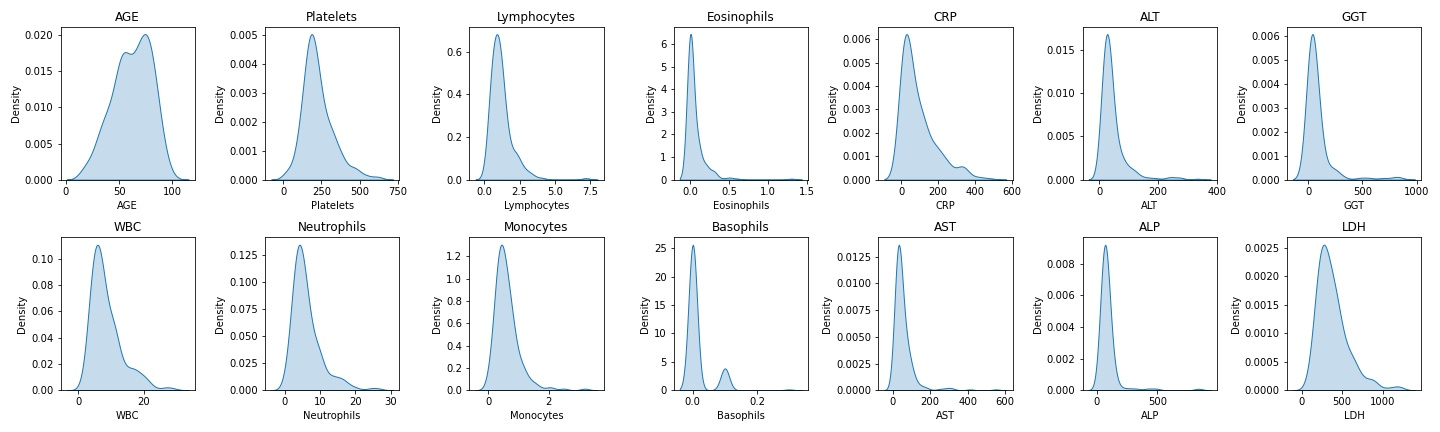
\includegraphics[width=1.1\textwidth]{density_no_split.jpg}
    \caption{Kernel density plots of the numerical features of the data set}
    \label{fig:density}
\end{figure}
\begin{figure}[ht]
 \centering
 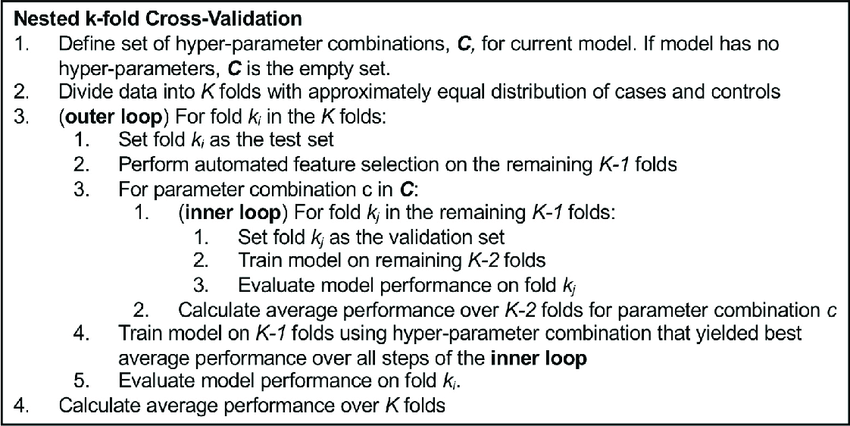
\includegraphics[width=1.1\textwidth]{k-fold-nested-cv.png}
 \caption{K-fold nested cross validation \cite{RN194}}
 \label{fig:cv}
\end{figure}
\begin{figure}
 \centering
 \begin{subfigure}{0.6\textwidth}
  \centering
  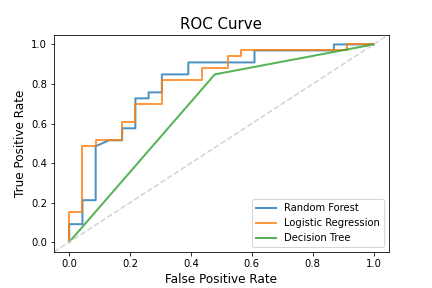
\includegraphics[width=\linewidth]{roc.png}
  \caption{Receiver Operating Characterisitcs (ROC) curve}
  \label{fig:roc}
 \end{subfigure}
 \begin{subfigure}{0.6\textwidth}
  \centering
  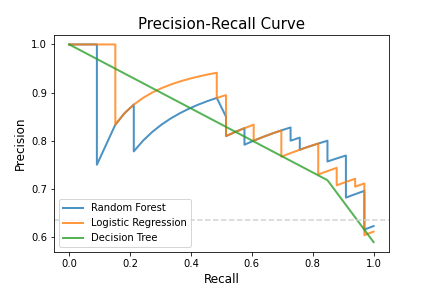
\includegraphics[width=\linewidth]{prc.png}
  \caption{Precision-Recall Curve}
  \label{fig:prc}
 \end{subfigure}
 \caption{ROC and Precision-Recall curve}
 \label{fig:prc-roc}
\end{figure}

\begin{figure}
 \begin{subfigure}{0.5\textwidth}
  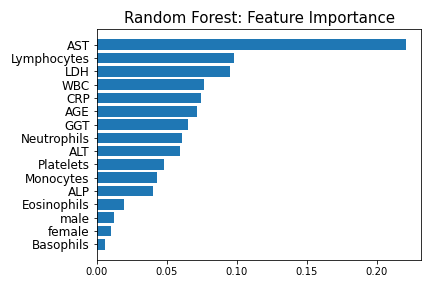
\includegraphics[width=\linewidth]{rf_importance.png}
  \caption{Random Forest}
  \label{fig:rf_importance}
 \end{subfigure}
 \begin{subfigure}{0.5\textwidth}
  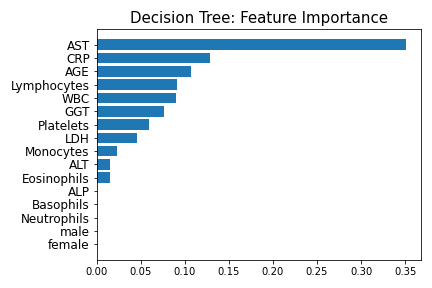
\includegraphics[width=\linewidth]{dt_importance.png}
  \caption{Decision Tree}
  \label{fig:dt_importance}
 \end{subfigure}
 \begin{subfigure}{\textwidth}
 \centering
  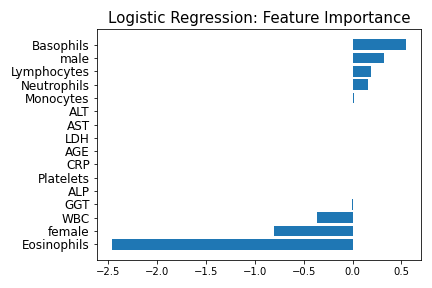
\includegraphics[width=0.5\linewidth]{lr_importance.png}
  \caption{Logistic Regression}
  \label{fig:lr_importance}
 \end{subfigure}
 \caption{Feature importance plots}
 \label{fig:feature-importance}
\end{figure}
\begin{figure}
 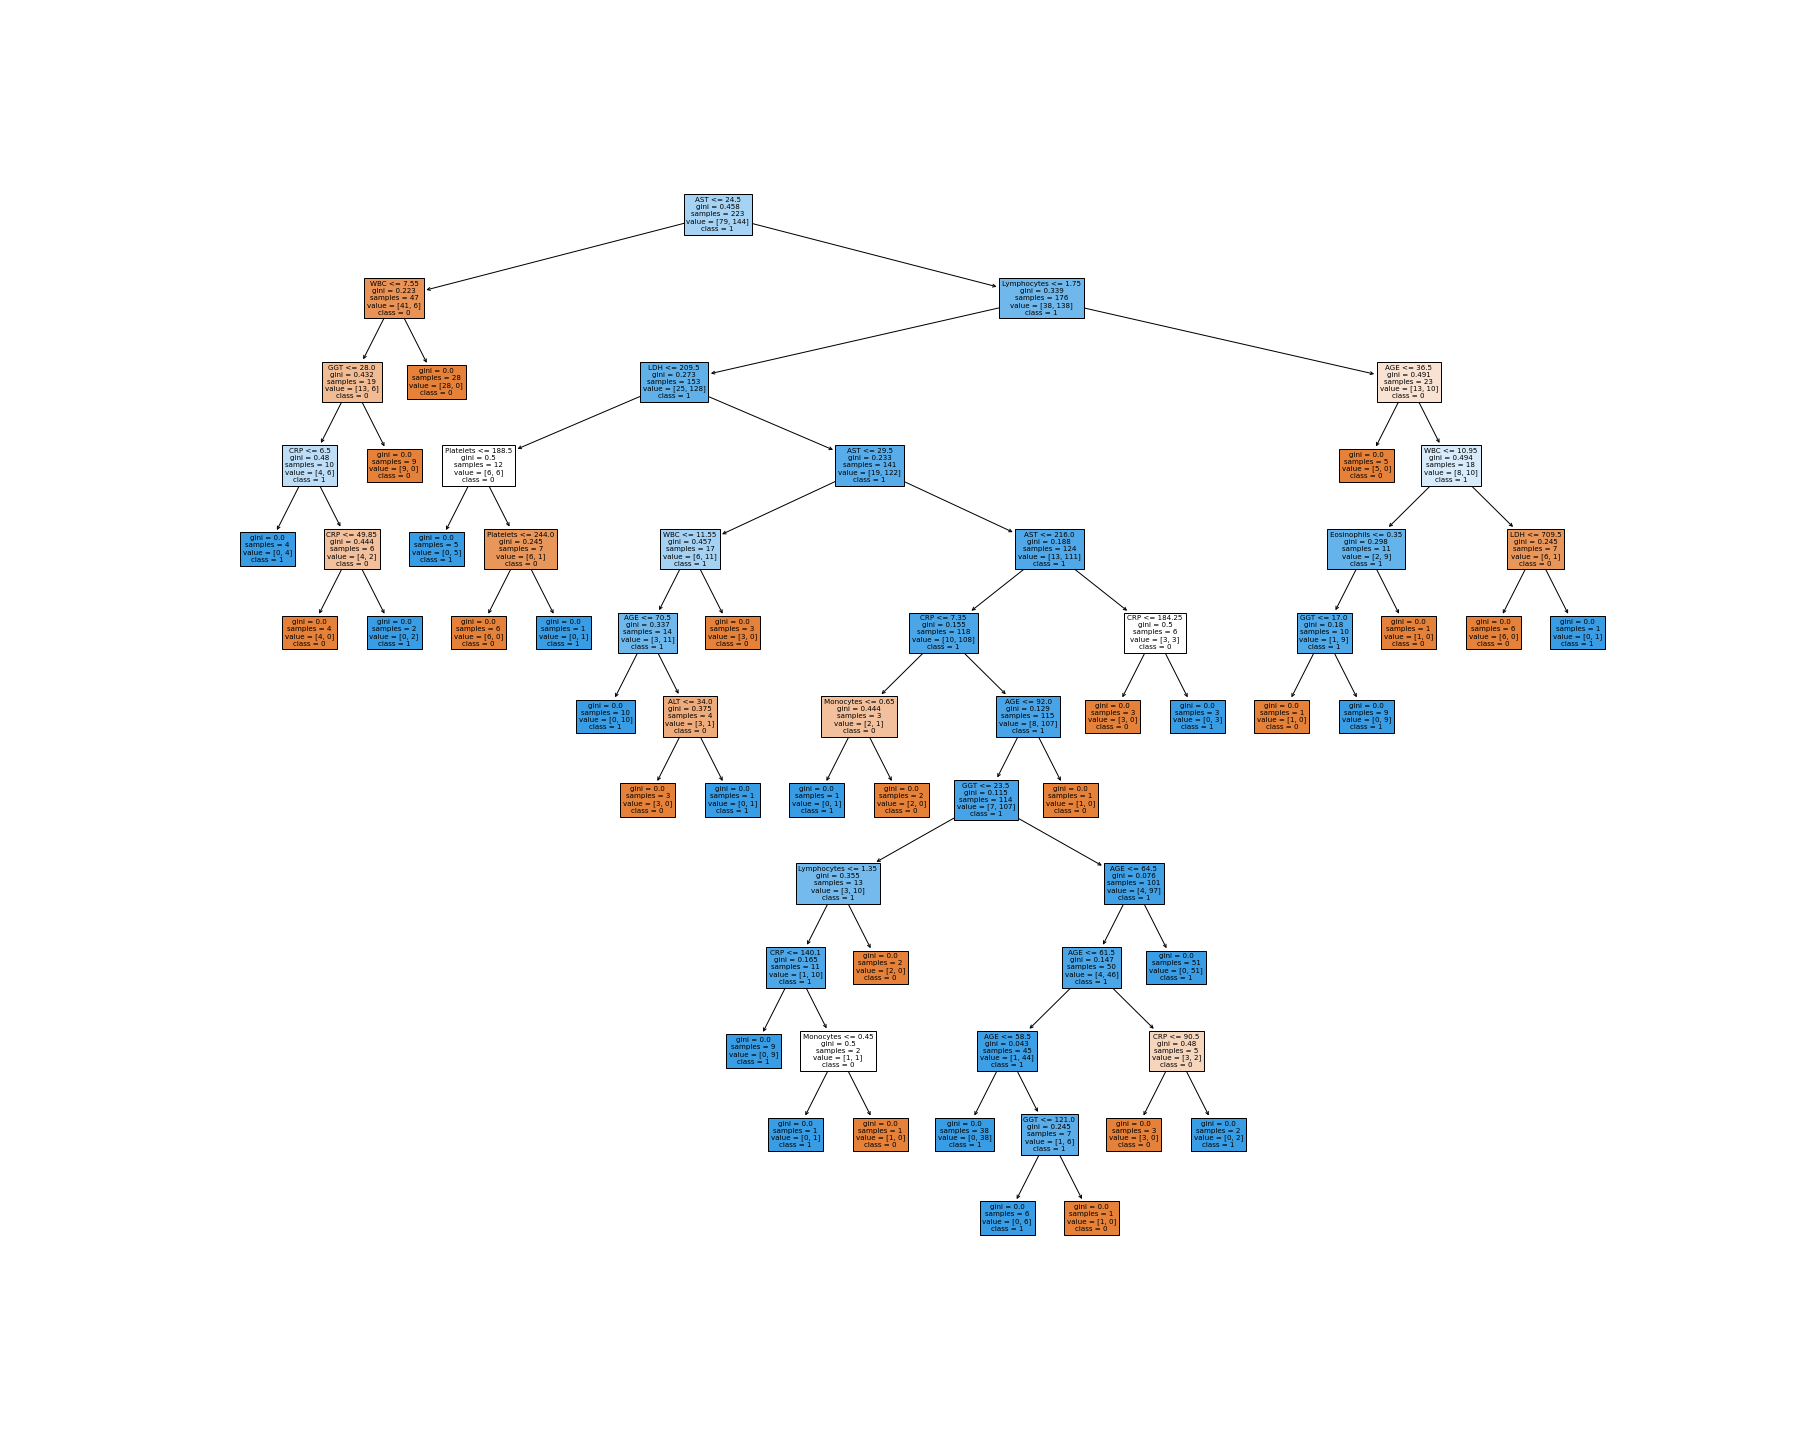
\includegraphics[width=1.5\textwidth, angle=90]{dt.png}
 \caption{Visualization of the Decision Tree produced during the validation 
phase}
 \label{fig:dt}
\end{figure}


